\documentclass{beamer}
\usepackage[utf8]{inputenc}
\usetheme{Warsaw}


\usepackage{tikz}
\usetikzlibrary{arrows}

\title{Nintendo Entertainment System}
\author{Jonathan Sieber}
\date[09.12.11]{09. Dez 2011}

        \institute{Betreuer: Dipl.-Ing. Benjamin Thielmann}

\begin{document}
    \begin{frame}
        \maketitle
        \begin{center}
%            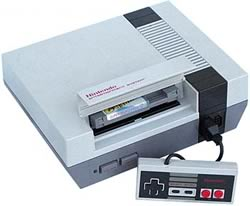
\includegraphics[height=0.4\textheight]{img/nes.jpg}
        \end{center}
    \end{frame}
    
    \begin{frame}
    \frametitle{Person}
    \begin{itemize}
        \item{Jonathan Sieber}
        \item{Informatikstudent im 7. Semester}
        \item{Seit 2007 freiberufliche Arbeit in Spieleentwicklung}
        \item{Mitarbeit an Landwirtschaftssimulator 2010, Demolition Company}
        \item{Besonderes Interesse an Systemprogrammierung, Portierung}
    \end{itemize}
    \end{frame}
    
    
    \begin{frame}
        \frametitle{Das Ziel}
        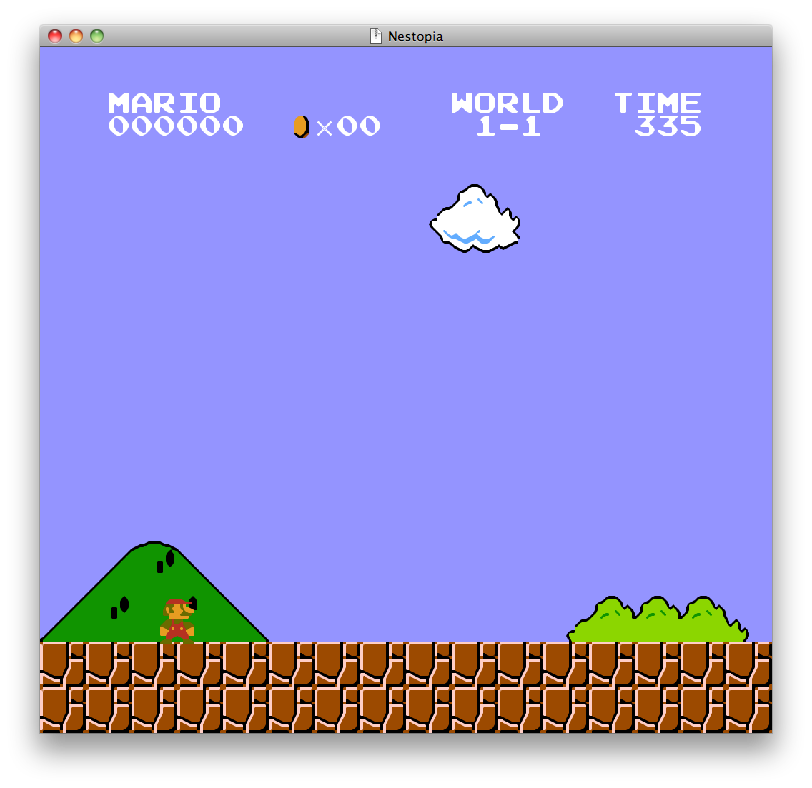
\includegraphics[width=0.8\linewidth]{img/smb.png}
    \end{frame}
    
    
        
    \begin{frame}
        \frametitle{Geschichte}
        \begin{columns}
             \column{.45\textwidth}
                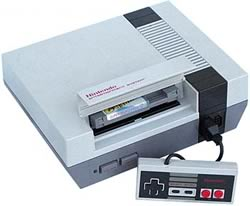
\includegraphics[width=1.1\textwidth]{img/nes.jpg}
                
             \column{.55\textwidth}
             
                \begin{itemize}
                    \item{1983 als Nintendo Famicom in Japan veröffentlicht}
                    \item{Spiele erschienen bis 1996}
                    \item{Große Fangemeinde und aktive Emulator-Szene}
                \end{itemize}
        \end{columns}
    \end{frame}
    
    
    \begin{frame}
        \frametitle{Hardwareübersicht}
        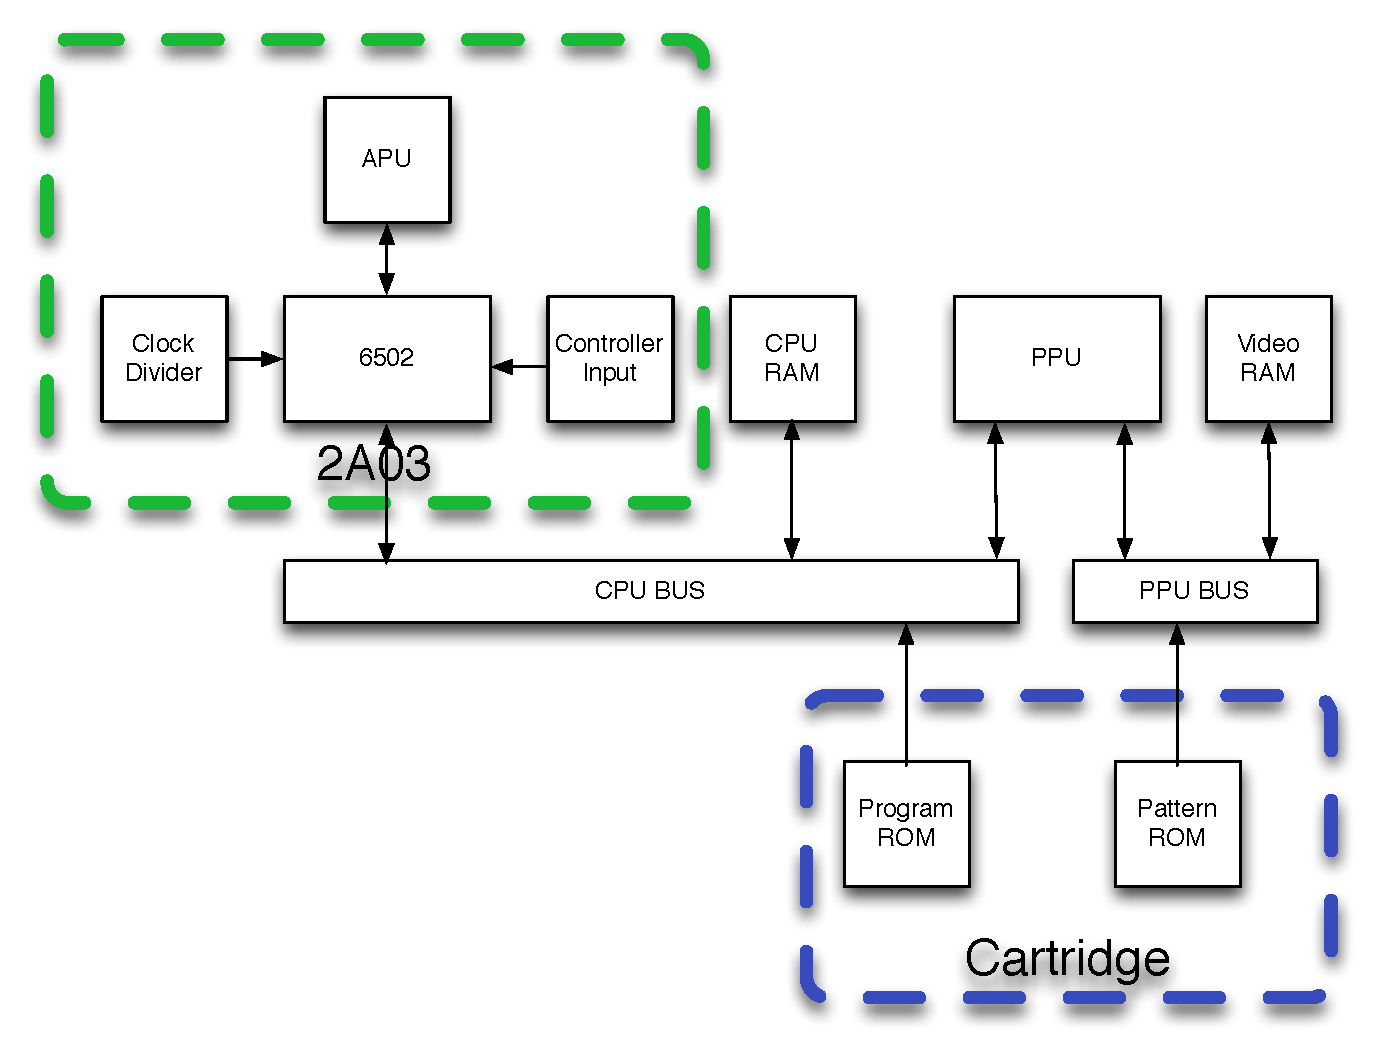
\includegraphics[width=0.8\textwidth]{img/system1.pdf}
    \end{frame}
    
    
    \begin{frame}
        \frametitle{CPU}
        \begin{itemize}
            \item{Custom Chip Ricoh 2A03 @ 1.76 MHz}
            \item{Basiert auf MOS Technology 6502}
            \item{Enthält Soundgenerator}
            \item{DMA-Einheit für Sprite-Updates auf PPU}
        \end{itemize}
    \end{frame}
    
    \begin{frame}
        \frametitle{PPU}
        \begin{itemize}
            \item{Ricoh RP2C02}
            \item{@5.37 Mhz = NTSC Pixel Clock}
            \item{1 Background Layer mit flüssigem Scrolling}
            \item{64 Sprites}
        \end{itemize}
    \end{frame}

    \begin{frame}
        \frametitle{Cartridges}
        \begin{itemize}
            \item{Direkt am Systembus angebundene Steckkarten}
            \item{32k Programmcode und 8k Grafikdaten direkt addressierbar}
            \item{Spätere Spiele benutzen wesentlich mehr}
        \end{itemize}
    \end{frame}
    
    \begin{frame}
        \frametitle{Moderne Umsetzung}
        \includegraphics<1>[width=0.8\textwidth]{img/system1.pdf}
        \includegraphics<2>[width=0.8\textwidth]{img/system2.pdf}
    \end{frame}
    
    \begin{frame}
        \frametitle{HDMI-Ausgabe}
        \begin{itemize}
            \item{HDMI Ausgabe}
            \item{Übernommen aus EDK-Modul xps\_tft}
            \item{256x240 Pixel Framebuffer im FPGA-internen Block-RAM}
            \item{Ausgabe auf 640x480}
            \item{Höhere Auflösung und bessere Skalierung geplant}
        \end{itemize}
    \end{frame}
    
    \begin{frame}
        \frametitle{System Aufbau für Super Mario Bros.}
        \begin{itemize}
            \item{Geräte am CPU-BUS zusammenhängen und multiplexen}
            \item{NES ROM Files für SMB einlesen und ROM beschreiben}
            \item{PPU und HDMIOut mit Framebuffer verbinden}
        \end{itemize}
    \end{frame}
    
        
    \begin{frame}
        \frametitle{Umsetzung CPU} 
        \begin{columns}
             \column{.45\textwidth}
                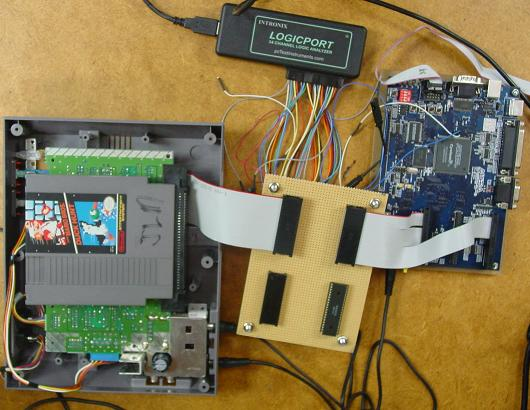
\includegraphics[width=1.1\textwidth]{img/danleach.jpg}
             \column{.55\textwidth}
                \begin{itemize}
                    \item{Master's Project von Dan Leach (Bradley University)}
                    \item{Ersetzt die CPU aus Original-Hardware}
                    \item{Basiert selbst auf 6502-Implementierung von fpgaarcade.com}
                    \item{Noch ohne Soundgenerator}
                \end{itemize}
        \end{columns}
    \end{frame}
    
    \begin{frame}
        \frametitle{Probleme}        
        \begin{columns}
             \column{.45\textwidth}
                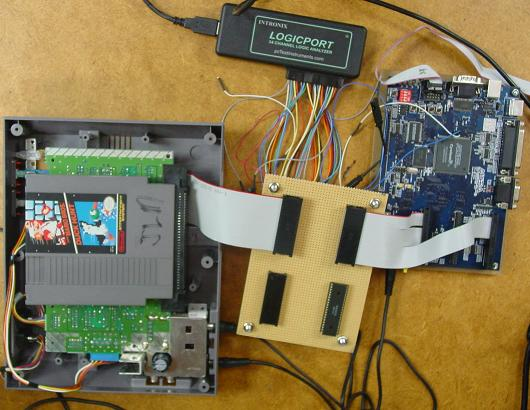
\includegraphics[width=1.1\textwidth]{img/danleach.jpg}
             \column{.55\textwidth}
                \begin{itemize}
                    \item{6502 verwendet mehrphasigen Clock}
                    \item{Clock Divider Konzept problematisch, kein DCM/PLL}
                    \item{Lief nicht nach der Synthese}
                    \item{Umbau auf Clock Enables}
                \end{itemize}
        \end{columns}
    \end{frame}
    
    
    \begin{frame}
        \frametitle{PPU Dokumentation}
        \begin{itemize}
            \item{Viel Doku aus Emulator-Szene}
            \item{Informelle Verhaltensbeschreibungen aller Komponenten}
            \item{Besonders viele wichtige Details zu PPU}
        \end{itemize}
    \end{frame}
    
    \begin{frame}
        \frametitle{Pattern Table}
         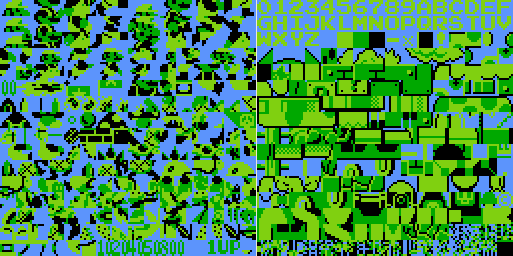
\includegraphics[height=0.5\linewidth]{img/pattern.png}   
        \begin{itemize}
                \item{Background-Tiles definieren Palette per 16x16 Pixel}
                \item{Sprites haben eigene Paletten}
                \item{Dies sind alle Grafiken aus Super Mario}
        \end{itemize}
    \end{frame}
    
    \begin{frame}
        \frametitle{Background Layer}
        \begin{columns}
             \column{.45\textwidth}
                 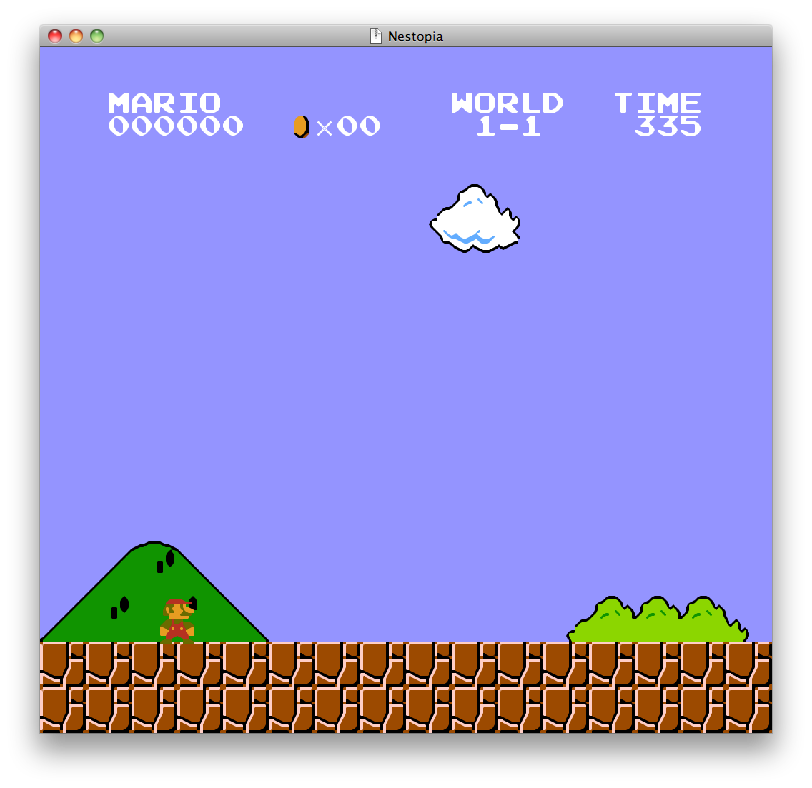
\includegraphics[width=1.1\textwidth]{img/smb_bg.png}                
             \column{.55\textwidth}             
                \begin{itemize}
                       \item{Lückenloser Hintergrund aus 32x30 Objekten}
                       \item{Für 16x16 Pixel je eine 4-Farben Palette}
                        \item{Pipeline mit geschickten Datenformaten braucht 4 Byte-Speicherzugriffe pro 8 Pixel}
                \end{itemize}
        \end{columns}
    \end{frame}
    
    \begin{frame}
        \frametitle{Sprite Layer}
        \begin{columns}
             \column{.45\textwidth}
                 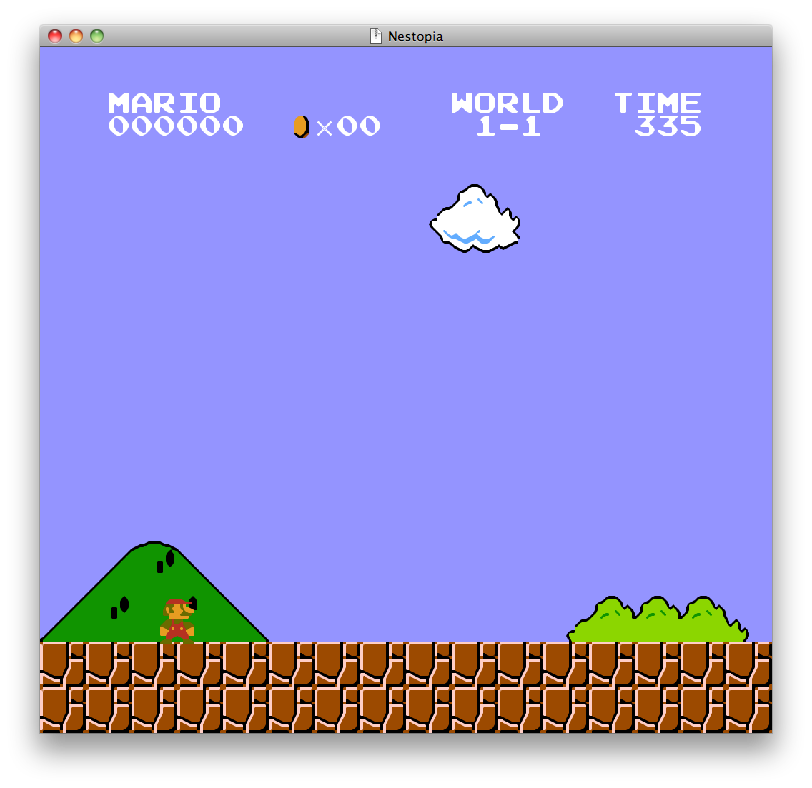
\includegraphics[width=1.1\textwidth]{img/smb_sprite.png}                
             \column{.55\textwidth}             
                \begin{itemize}
                        \item{Frei bewegliche Objekte mit 8x8 oder 8x16 Pixeln}
                        \item{Bis zu 64 Sprites gleichzeitig}
                        \item{Werden in der HSYNC-Lücke prefetched, daher nur 8 Sprites pro Zeile}
                \end{itemize}
        \end{columns}
    \end{frame}
    
    
    \begin{frame}
        \frametitle{Hardwareübersicht}
        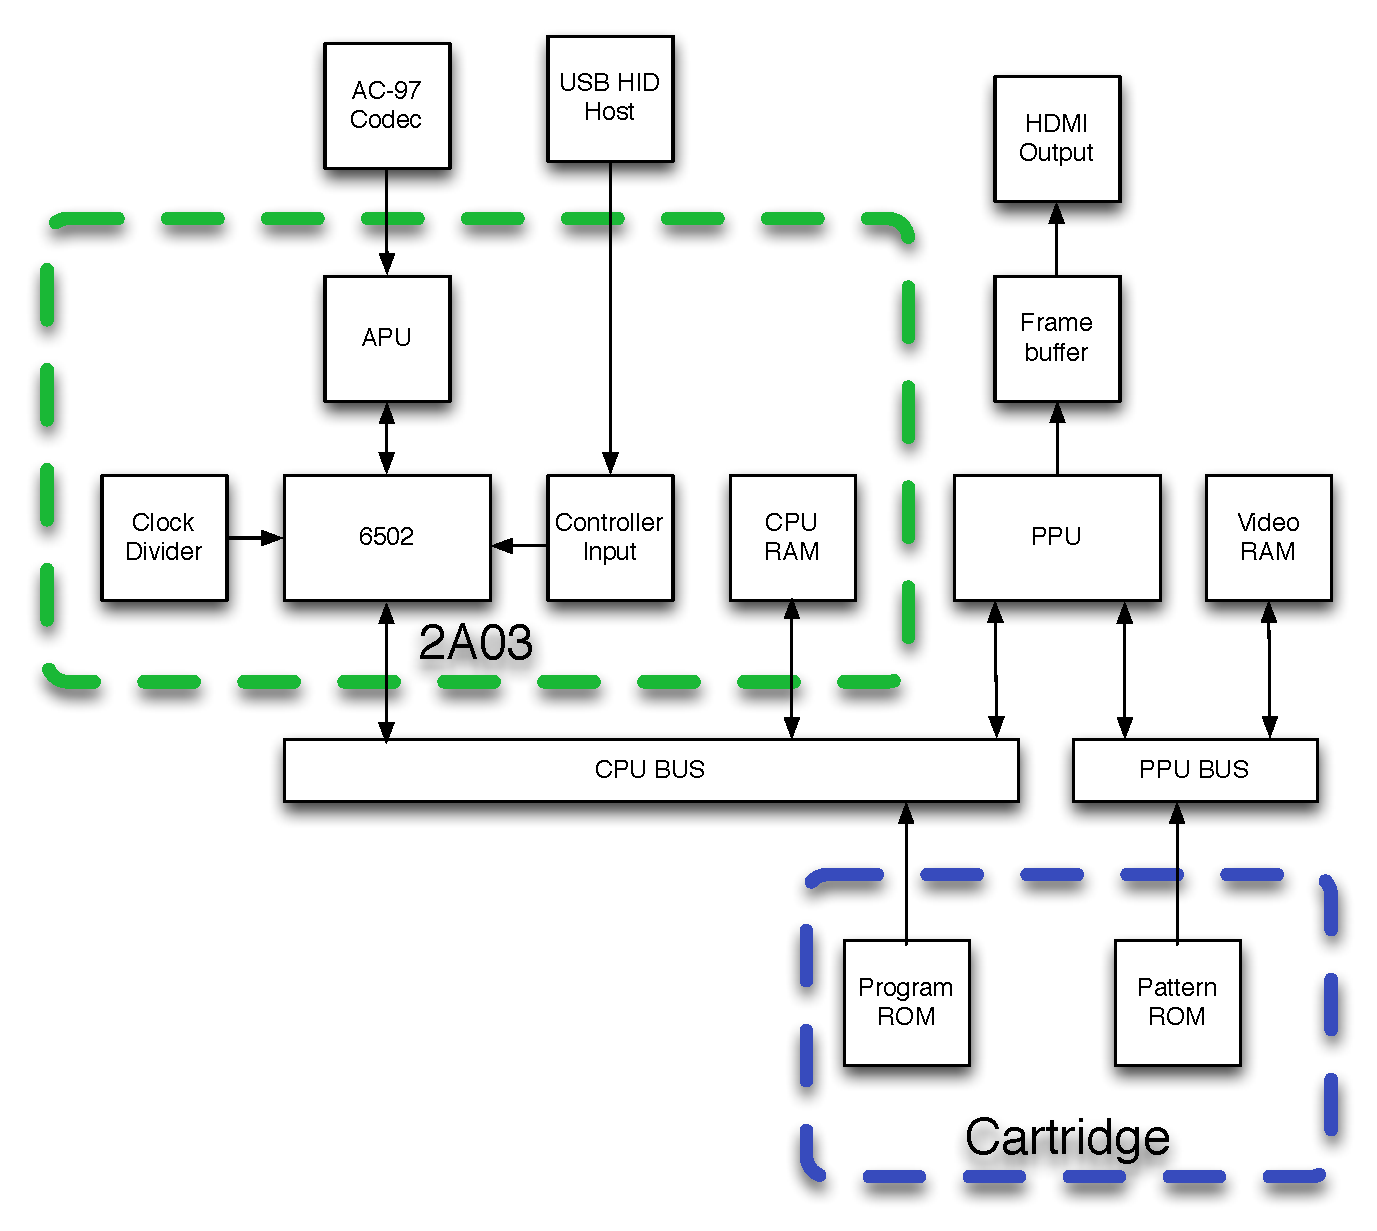
\includegraphics[width=0.8\textwidth]{img/system2.pdf}
    \end{frame}
    
    \begin{frame}
        \frametitle{Hardwareübersicht}
        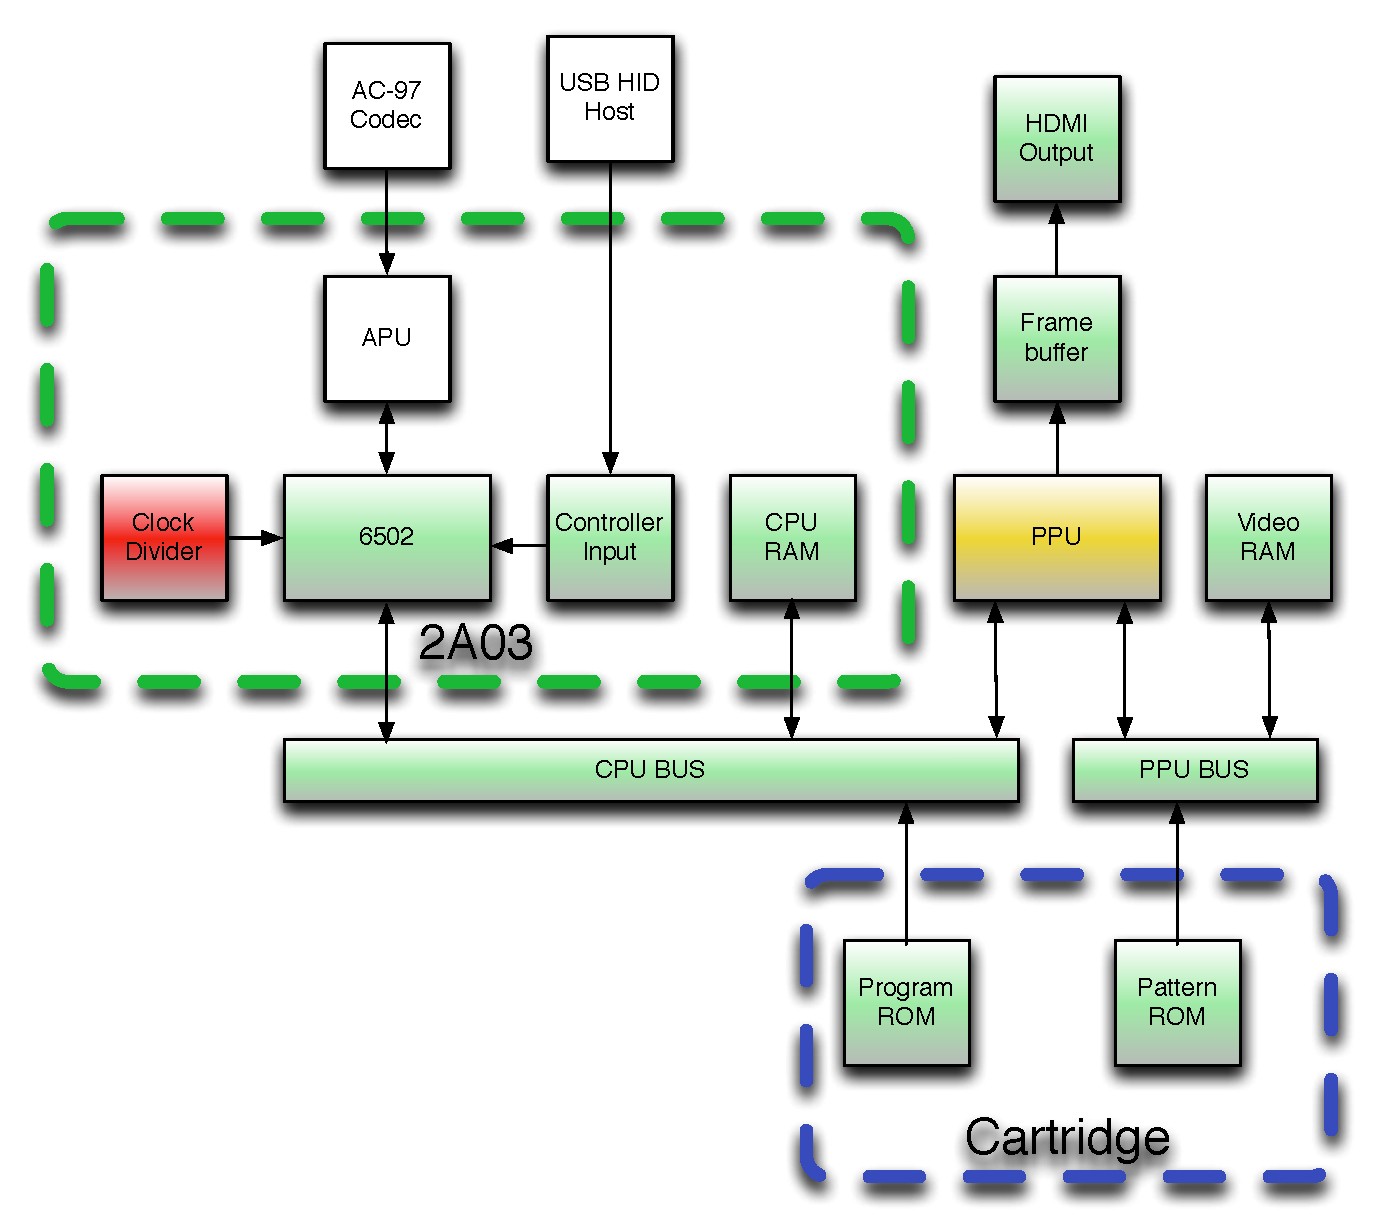
\includegraphics[width=0.8\textwidth]{img/system3.pdf}
    \end{frame}
    
   
    \begin{frame}
        \frametitle{Ende}
        \begin{itemize}
            \item{Fragen?}
        \end{itemize}
    \end{frame}
    

\end{document}
